\documentclass[12pt]{article}
\usepackage{fullpage}
\usepackage{graphicx}
\usepackage{hyperref}
\begin{document}

\title{Unsupervised Signature Detection in USPTO PAIR Scans}
\author{Gabe Fierro}
\date{\today}
\maketitle

\section{Introduction}

Social science research into technological innovation and economic trends oft makes use of analyzing patent data. Raw, digital patent data dating back to 1976 is distributed by the US Patent and Trademark Office (USPTO), which updates the repository weekly with new records. However, detailed research is hampered by the the fact that the raw patent data is rife with errors and lacks unique identifiers of common records. Inventors with multiple patents will often have inconsistent metadata across records, including misspellings of names, changing surnames, inclusion or omission of middle names, different locations and having innovations in differing technological domains. Work has been done into inventor-level disambiguation of patent data, but the inherent noise of the data makes it difficult to achieve greater than around 95\% accuracy. Simply put, there's only so well we can do with the current raw patent data.
%need citations
The Patent Application Information Retrieval (PAIR) documents available through the USPTO offer an additional wealth of information concerning patent applications. To complement the data-driven inventor disambiguation, we explore extracting signatures from the scanned PAIR documents, associate the signatures with inventor names, and use this additional data to better associate inventor records. 

\section{Using PAIR Data}

\begin{figure}
\center
\begin{tabular}{| l | l | l |}
\hline
Document Code & Document Description & Signature Found \\
\hline
OATH & Oath or Declaration filed  & Inventor \\
TRNA & Transmittal of New Application & Lawyer \\
PET & Petition Entered & Usually Inventor \\ 
PETDEC & Petition Decision & Patent Examiner \\ 
\hline
\end{tabular}
\caption{Table of some of the common document types found in Image File Wrappers}
\label{fig:documenttypes}
\end{figure}

The public PAIR data itself comprises around 5,239,432 records as of 11 September, 2013. %http://www.google.com/googlebooks/uspto-patents-pair.html
While the public PAIR data is not available for the full range of USPTO digital patent records (1975 through 2013), it provides information on denied and abandoned as well as granted applications.
The PAIR data contains ample metadata concerning each application. The Image File Wrapper for an application contains scans of the documents sent between the patent examiner and the patent applicant as part of the application process. 

Several types of documents included in the Image File Wrapper contain the signatures of the patent examiner, patent inventors and lawyers. This raises the problem of identifying to which individual a signature belongs. The naive approach of performing optical character recognition (OCR) on the document and then semantically determining the signer of a document is cumbersome and too time consuming to be tractable. We can pare down the document space by pre-identifying the types of documents that are more likely to contain signatures by one of the relevant parties. Some of these documents can be found in Figure ~\ref{fig:documenttypes}.

Most documents will contain only one signature, which can easily be attributed to either the inventor, lawyer or examiner by pairing the document type with pre-existing digital patent metadata, which does not require further processing of the document.

\section{Signature Detection}

\begin{figure}
\center
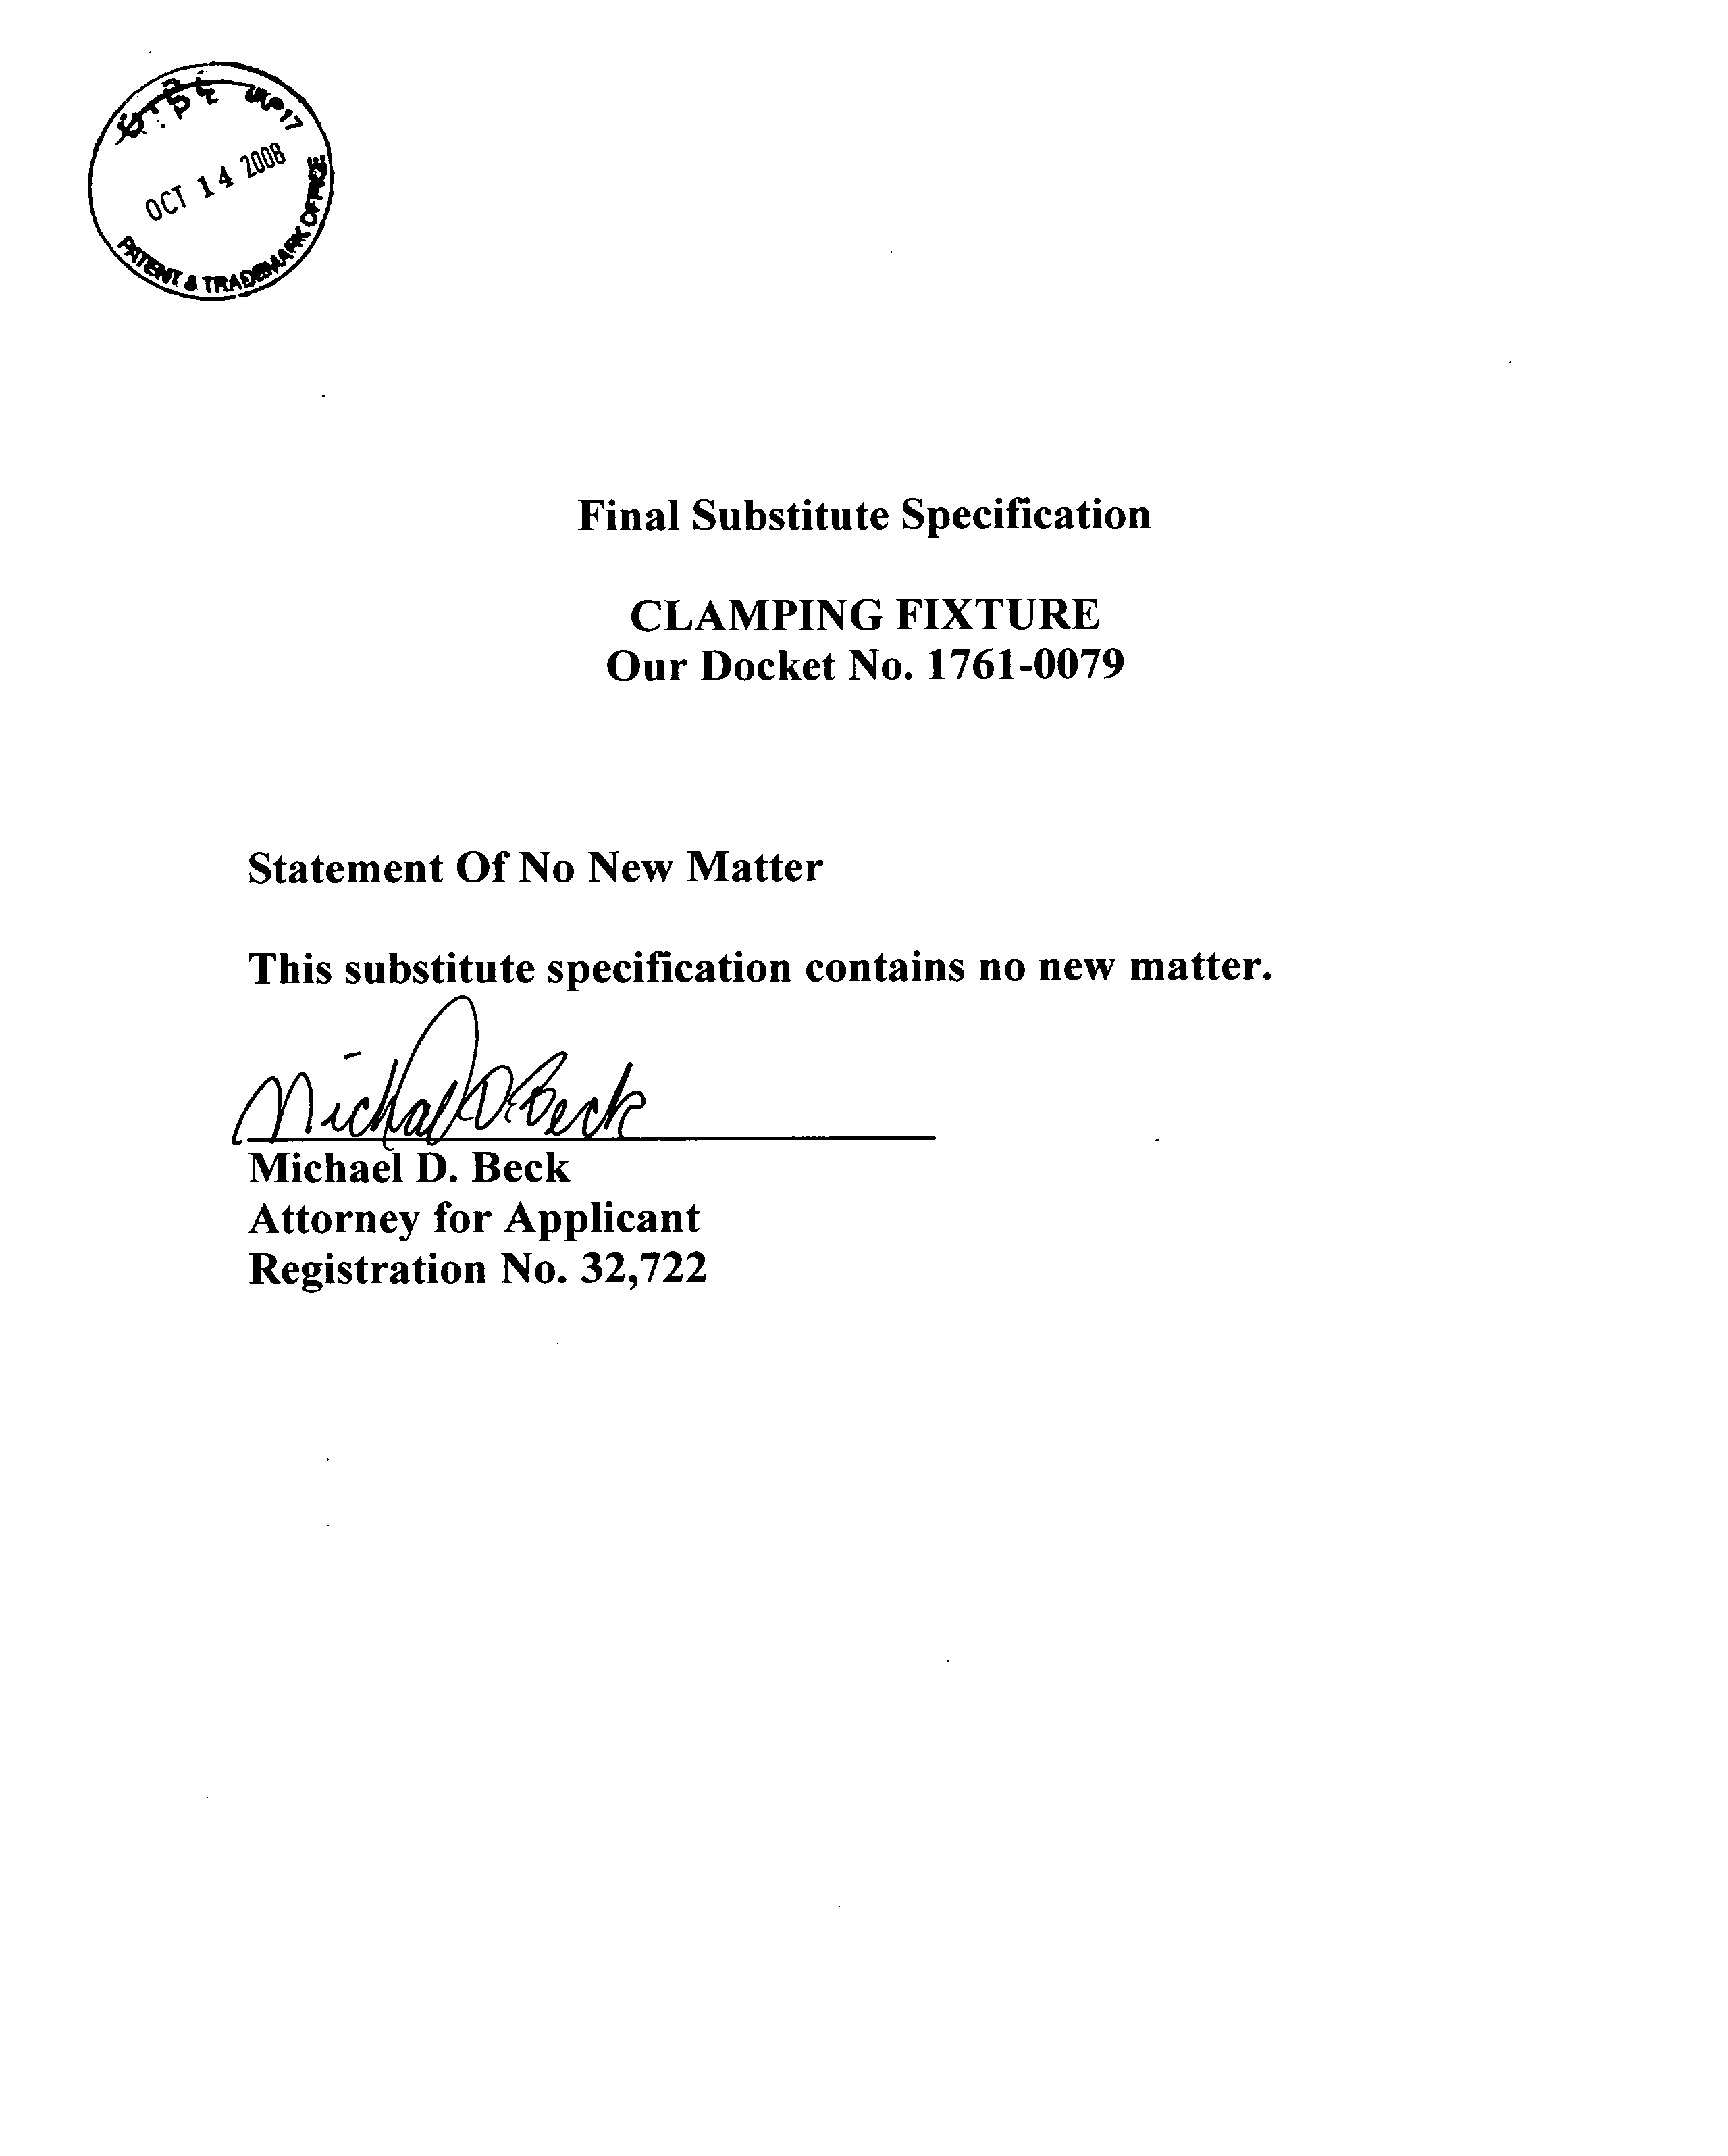
\includegraphics[scale=.5, trim=0 4in 0 3in, clip=true]{figs/signature2}
\caption{Example scanned document containing the applicant's lawyer's signature and name}
\end{figure}

There are two initial tasks that must be accomplished: the detection and extraction of the signature, and the detection and extraction of the applicant's name. Unlike most traditional computer vision tasks, there is no defined training set for `teaching' an application how to appropriately extract the requisite information. However, we can simplify these two tasks by virtue of having documents that follow fairly predictable patterns.

The document scans are fairly high quality, with little to no superfluous marks, containing mostly text, the occasional seal (a circular logo), and signatures. When signatures do appear, they appear on a flat line and consist mostly of long connected curves. This allows us to use known methods to find contours in an image. The longer these contours are, the more likely they are part of a signature. We've found that only taking contours longer than 300 pixels is a good lower bound.

\begin{figure}
\center
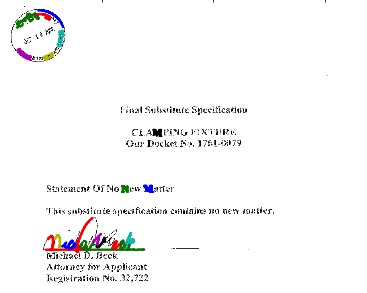
\includegraphics{figs/contour-detection}
\caption{Example of contour detection. Note the signature has been highlighted, but there are also several false matches in the document, most notably the seal in the top left. Different colors represent separate contours.}
\end{figure}

Once we have a set of contours for a document, we compute the centroids of each of these contours to get a rough sense of how they are clustered. We run the DBSCAN (\url{https://en.wikipedia.org/wiki/DBSCAN}) algorithm to identify clusters of points that exhibit a similar density to what we would expect for a signature. For each of the found clusters, we run a simple linear regression on the points. The cluster with the lowest error and the most horizontal slope is most likely the signature.

\begin{figure}
\center
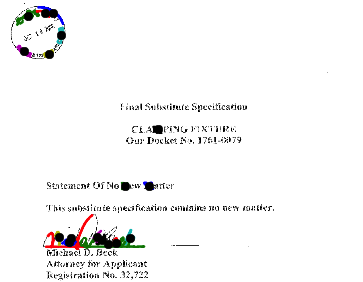
\includegraphics{figs/contour-centroid}
\caption{Example of computing centroids (black dots) for each of the contours. Note how the centroids on the signature form a rough line.} 
\end{figure}

\begin{figure}
\center
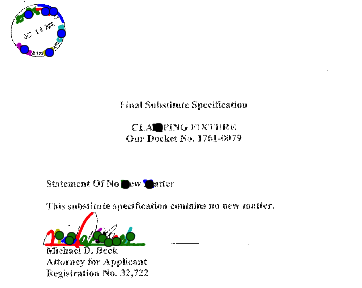
\includegraphics{figs/contour-dbscan}
\caption{Running the DBSCAN algorithm on the contour centroids. Centroids of the same color are considered to be in the same cluster. Note the centroids in the signature are all considered part of the same cluster.}
\end{figure}

\begin{figure}
\center
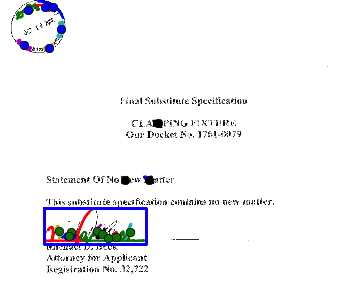
\includegraphics{figs/boundingbox}
\caption{By finding the most closely horizontal group of points, we can draw a bounding box around the corresponding contours and find the signature}
\end{figure}

%TODO: get stats on how often signatures appear
%\newpage
%{
%\scriptsize
%\bibliographystyle{acm}
%\bibliography{signature_detection}
%}

\end{document}
